\chapter{Builder Pattern}

\section{Định nghĩa}
Builder Pattern là một trong những Creational pattern. Builder Pattern là mẫu thiết kế đối tượng được tạo ra để xây dựng một đối tượng phức tạp bằng cách sử dụng các đối tượng đơn giản và sử dụng tiếp cận từng bước, việc xây dựng các đối tượng độc lập với các đối tượng khác. Builder Pattern được xây dựng để khắc phục một số nhược điểm của Factory Pattern và Abstract Factory Pattern khi mà Object có nhiều thuộc tính (các nhược điểm đó là: quá nhiều tham số phải truyền vào từ phía client tới Factory Class; một số tham số có thể là tùy chọn nhưng trong Factory Pattern, chúng ta phải gửi tất cả tham số, với tham số tùy chọn nếu không nhập gì thì sẽ truyền là null; nếu một Object có quá nhiều thuộc tính thì việc tạo sẽ phức tạp).

\section{Mục đích sử dụng}
\begin{itemize}
\item Tạo một đối tượng phức tạp: có nhiều thuộc tính (nhiều hơn 4) và một số bắt buộc (requried), một số không bắt buộc (optional).
\item Tách rời quá trình xây dựng một đối tượng phức tạp từ các phần tạo nên đối tượng.
\item Kiểm soát quá trình xây dựng.
\item Tạo nhiều cách khác nhau cho đối tượng được xây dựng.
\end{itemize}

\section{Mô hình cấu trúc}
\begin{center}
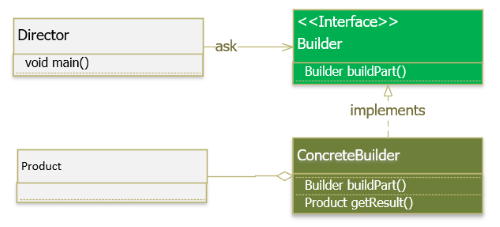
\includegraphics{GALLEYS/images/chapter10/diagram}
\end{center}
Các thành phần cơ bản:\\
\begin{itemize}
\item Product : đại diện cho đối tượng cần tạo, đối tượng này phức tạp, có nhiều thuộc tính.
\item Builder : là abstract class hoặc interface khai báo phương thức tạo đối tượng.
\item ConcreteBuilder : kế thừa Builder và cài đặt chi tiết cách tạo ra đối tượng. Nó sẽ xác định và nắm giữ các thể hiện mà nó tạo ra, đồng thời nó cũng cung cấp phương thức để trả các các thể hiện mà nó đã tạo ra trước đó.
\item Director/Client: là nơi sẽ gọi tới Builder để tạo ra đối tượng.
\end{itemize}
Trường hợp đơn giản, chúng ta có thể gộp Builder và ConcreteBuilder thành static nested class bên trong Product.\\

Ta xét một ví dụ cụ thể: Tạo một static nested class (đây được gọi là builder class) và copy tất cả các tham số từ class bên ngoài vào. Chúng ta nên đặt tên của static nested class này theo định dạng là tên class + Builder. Ví dụ class là Computer thì builder class sẽ là ComputerBuilder. Class Builder có một hàm khởi tạo public với tất cả các thuộc tính bắt buộc, ngoài ra còn có các method setter cho các tham số tùy chọn. Cung cấp method build() trong Class Builder để trả về đối tượng mà client cần.
\begin{center}
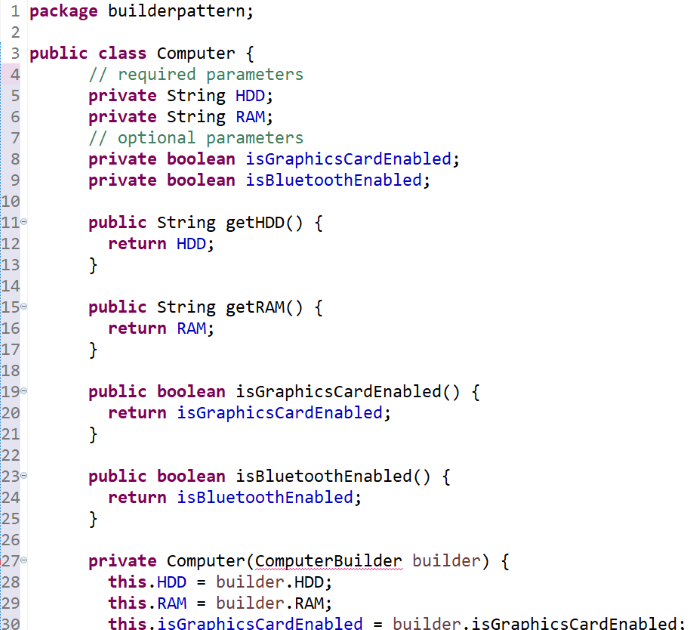
\includegraphics{GALLEYS/images/chapter10/code1}
\end{center}
\begin{center}
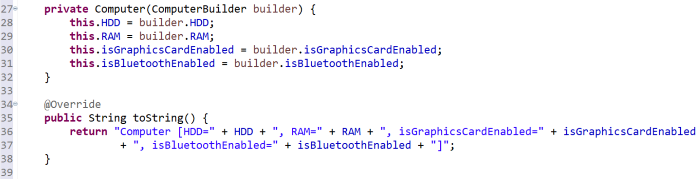
\includegraphics{GALLEYS/images/chapter10/code2}
\end{center}
\begin{center}
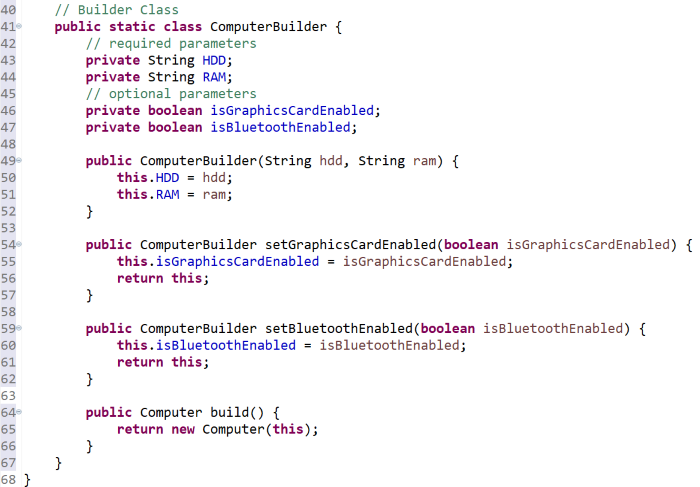
\includegraphics{GALLEYS/images/chapter10/code3}
\end{center}
Class Computer.java chỉ có method getter và không có hàm khởi tạo public nên chỉ có một cách duy nhất để lấy một đối tượng Computer là thông qua class ComputerBuilder.\\
\newpage
\textbf{Demo:}
\begin{center}
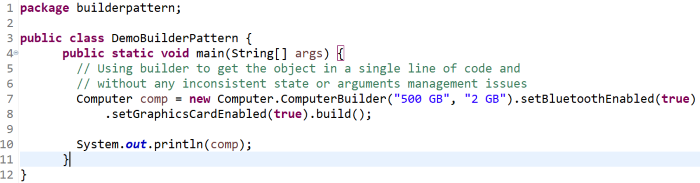
\includegraphics{GALLEYS/images/chapter10/code4}
\end{center}
\textbf{Và chúng ta có được kết quả:}
\begin{center}
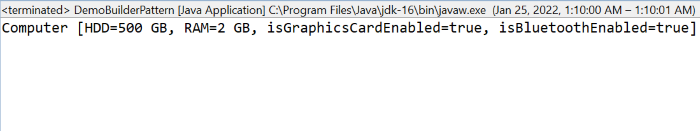
\includegraphics{GALLEYS/images/chapter10/code5}
\end{center}
Tương tự, thay vì tạo nested static class ComputerBuilder bên trong class Computer chúng ta có thể định nghĩa nó thành 1 class riêng như mô hình UML ở trên.

\section{Builder Pattern trong thực tế}
Một số ví dụ sử dụng Buider Pattern trong JDK:
\begin{itemize}
\item java.lang.StringBuilder.append()
\item java.lang.StringBuffer.append()
\end{itemize}
Một ví dụ về việc sử dụng Builder khác là xây dựng một tài liệu XML. Ngoài ra Builder Pattern cũng có những ứng dụng thực tế khác khá gần gũi, như cho việc gọi món tại một cửa hàng thức ăn nhanh (trên một phần mềm nào đó).